\documentclass{beamer}

\usepackage{graphicx,hyperref,url}
\usepackage[utf8]{inputenc}
\usepackage[T1]{fontenc}
\usepackage{booktabs}
\usepackage[portuges]{babel}
\usepackage{lmodern, comment}
\usepackage{xcolor}
\usepackage{pifont}
\usepackage[final]{listings}
%%\usepackage{udesc} 

%%% FIGS \graphicspath{{figures/}{../figures/}{C:/Users/me/Documents/project/figures/}}

\graphicspath{ {figures/} {../ia_combinatoria/figures/} }
%%%%\graphicspath{ {/home/user} }
\definecolor{azulclaro}{rgb}{0.9,0.9,0.9}
\definecolor{mygreen}{rgb}{0,0.6,0}
\definecolor{mygray}{rgb}{0.5,0.5,0.5}
\definecolor{mymauve}{rgb}{0.58,0,0.82}
\definecolor{darkgray}{rgb}{.4,.4,.4}
\definecolor{purple}{rgb}{0.65, 0.12, 0.82}


\lstset{ 
  %  label={pgm_ex01},
    backgroundcolor=\color{azulclaro}, 
    language=Haskell, %%Miranda,%%Perl,%%%Python, %%Mercury,
    showstringspaces=false,
    basicstyle=\bf\scriptsize\ttfamily,
%%      basicstyle= \footnotesize %%% TESTAR
%%      keywordstyle=\bfseries\color{green!40!black},
    keywordstyle=\textbf{\color{mygreen}}, 
    otherkeywords={*, \%, array, constraint, solve, output,  show, "/\", satisfy, set, of, if, then, elseif, float, search},
%%  keywordstyle=\color{blue},       % keyword style
%%    commentstyle=\itshape\color{purple!40!black},
      commentstyle=\color{orange},    % comment style
      identifierstyle=\color{blue},
      stringstyle=\color{orange},
      stringstyle=\color{mymauve},
      numbers=left,  % where to put the line-numbers; possible values are (none, left, right)
      numbersep=5pt,   % how far the line-numbers are from the code
      numberstyle=\tiny\color{magenta},
      keepspaces=true      
    % %caption={LEGENDA no source PASCAL ficou OK},
}



\title[Inteligência Artificial -- Otimização Combinatória] % (optional, use only with long paper titlebg=blue!20!white,s)
{Inteligência Artificial, Otimização Combinatória: \\ Um Exemplo\\
Cabo de Guerra}

%\subtitle
%{About some things}

\author[Claudio Cesar de Sá] % (optional, use only with lots of authors)
{Claudio Cesar de Sá\inst{1}}
% - Give the names in the same order as the appear in the paper.
% - Use the \inst{?} command only if the authors have different
%   affiliation.

\institute[UDESC]{
    Departamento de Ci\^encia da Computa\c{c}\~ao \\
    Centro de Ci\^encias e Tecnol\'ogias\\
Universidade do Estado de Santa Catarina}
%  Departamento de Ciência da Computação -- DCC\\
%  Centro de Ciências Tecnológicas -- CCT\\
% Universidade do Estado de Santa Catarina -- UDESC

% - Use the \inst command only if there are several affiliations.
% - Keep it simple, no one is interested in your street address.

\date[30 ago 2016] % (optional, should be abbreviation of conference name)


\begin{document}

\begin{frame}
  \titlepage
\end{frame}



% Structuring a talk is a difficult task and the following structure
% may not be suitable. Here are some rules that apply for this
% solution: 

% - Exactly two or three sections (other than the summary).
% - At *most* three subsections per section.
% - Talk about 30s to 2min per frame. So there should be between about
%   15 and 30 frames, all told.

% - A conference audience is likely to know very little of what you
%   are going to talk about. So *simplify*!
% - In a 20min talk, getting the main ideas across is hard
%   enough. Leave out details, even if it means being less precise than
%   you think necessary.
% - If you omit details that are vital to the proof/implementation,
%   just say so once. Everybody will be happy with that.

%%%%%%%%%%%%%%%%%%%%%%%%%%%%%%%%%%%%%%%%%%%%%%%%%%%%%%%


\begin{frame}

\begin{block}{Agenda}
%  \tableofcontents

\begin{enumerate}
  \item  Um sobrevôo na IA
  \item  O  que é complexidade computacional?
  \item  Um sobrevôo em otimização
  \item  Um exemplo: modelagem, código e resultados
  \item  Tendências
\end{enumerate}

\end{block}

\end{frame}


%%%%%%%%%%%%%%%%%%%%%%%%%%%%%%%%%%%%%%%%%%%%%%%%%%%%%%%
\begin{comment}
\section{Para efeitos de TEMPLATE}
\begin{frame}
\frametitle{Nome do SLIDE}
\begin{block}{Nome do Bloco}
  \begin{itemize}
   \item T1

    \item<2-> T2

    \item<3-> T3

  \item<4-> 

    \item<5-> 
    
        \item<6-> 
    \end{itemize}
  
\end{block}

\end{frame}
\end{comment}
%%%%%%%%%%%%%%%%%%%%%%%%%%%%%%%%%%%%%%%%%%%%%%%%%%%%%%%

%%%%%%%%%%%%%%%%%%%%%%%%%%%%%%%%%%%%%%%%%%%%%%%%%%%%%%%%%
\subsection{Áreas e Sucesso da IA}
\begin{frame}
\frametitle{Principais Áreas da IA}

\begin{figure}[ht!]
 \centering
 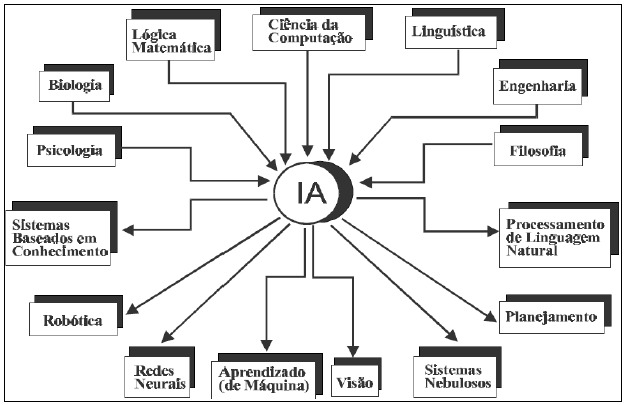
\includegraphics[width=0.9\textwidth , height=0.7\textheight]{../ia_combinatoria/figures/areas_da_IA.jpg}

\caption{Observe o sentido das setas !}

\end{figure}



\end{frame}



\subsection{IA $\times $ Otimização Combinatória (OC)}

\begin{frame}[fragile]
\frametitle{IA $\times $ Otimização Combinatória (OC)}

\begin{block}{IA $\Leftrightarrow $ OC:}
  \begin{itemize}
   \item  Ambas as áreas abordam problemas complexos!

    \item IA: diversas direções e muitos paradigmas

    \item Otimização Combinatória (OC): usa modelos como a IA, rígidos, espaços definidos ...
    
        \item A área de \textbf{Otimização} tem uma divisão: \textbf{Discreta} ou \textbf{Combinatória} e 
        \textbf{Contínua} ou \textbf{Numérica} (\textcolor{red}{não é o foco} -- funções deriváveis)
        
        \item  Atacar problemas difíceis! Contudo, o que é \textit{difícil}?
        
%        \item  Aqui: complexo $\approx $ difícil
                
       \item   Vamos definir \textit{uma medida de \textbf{complexo}}
    \end{itemize}
  
  \end{block}

\end{frame}



%%%%%%%%%%%%%%%%%%%%%%%%%%%%%%%%%%%%%%%%%%%%%%%%%%%%%%%
\section{Medindo a Complexidade}

\begin{frame}
\begin{block}{Definindo uma Medida Complexidade}
  \begin{itemize}
 
  \item Na área de CC tem uma medida clássica
  \item Classificar os problemas em \textbf{polinomiais} e \textbf{exponenciais}
     
     \item Assim, os problemas  \textbf{exponenciais} são os mais intrigantes ...
     \item O que é isto?
  \end{itemize}
\end{block}
\end{frame}


%%%%%%%%%%%%%%%%%%%%%%%%%%%%%%%%%%%%%%%%%%%%%%%%%%%%%%%
\subsection{Problema da Satisfatibilidade}

\begin{frame}
\frametitle{Problema da Satisfatibilidade}

\begin{block}{Fórmulas Lógicas}

Seja uma fórmula $\varphi_1 (x)$ sobre  o domínio $\{0 , 1\}$,
temos a sua interpretação dada Tabela Verdade abaixo:
$$
\begin{array}{c|c}
x & \varphi_1 (x)\\\hline
1 & \mathbf{1}\\
0 & \mathbf{0}
\end{array}
$$
% A \cdot \overline{B} + \overline{A} \cdot B and (A + B) \cdot ( \overline A + \overline B )
\end{block}

\end{frame}


\begin{frame}
\frametitle{Árvore semântica}
\begin{figure}[ht!]
 \centering
 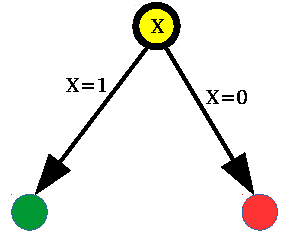
\includegraphics[width=0.4\textwidth , height=0.6\textheight]{x_tree.pdf}
\caption{Representando as validades da função $\varphi_1 (x)$} 
%\label{}
\end{figure}

\end{frame}

%%%%%%%%%%%%%%%%%%%%%%%%%%%%%%%%%%%%%%%%%%%%%%%%%%%%%%%%%%%%%%%%%%%%

\begin{frame}
\begin{block}{Fórmulas Lógicas}


Seja uma fórmula $\varphi_2 (x,y) = (\sim x \wedge y)\vee (x \wedge \sim y)$ 
sobre  o domínio $\{0 , 1\}$,
temos a sua interpretação dada Tabela Verdade abaixo:

$$
\begin{array}{cc|c@{}cccc@{}ccc@{}cccc@{}c | c}
x & y & ( &\lnot&x&\land&y&)&\lor&(&x&\land&\lnot&y&) & \varphi_2 (x,y) \\ \hline
1&1&&0&1&0&1&&\mathbf{0}&&1&0&0&1& & \mathbf{0}  \\
1&0&&0&1&0&0&&\mathbf{1}&&1&1&1&0& & \mathbf{1} \\
0&1&&1&0&1&1&&\mathbf{1}&&0&0&0&1& & \mathbf{1} \\
0&0&&1&0&0&0&&\mathbf{0}&&0&0&1&0& & \mathbf{0}
\end{array}
$$
%%%%((p \to q) \land (r \to s) \land (p \lor r)) 
%%%% (~x|y)&(~z|w)&(x|z)

\end{block}

\end{frame}

\begin{frame}
\frametitle{Sua árvore semântica é dada por:}

\begin{figure}[ht!]
 \centering
 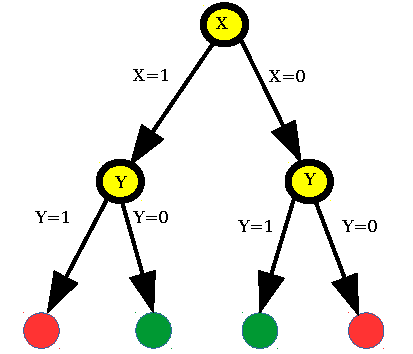
\includegraphics[width=0.8\textwidth , height=0.65\textheight]{xy_tree.pdf}
 \caption{Representando as validades da função $\varphi_2 (x,y)$} 
%\label{}
\end{figure}

\end{frame}
%%%%%%%%%%%%%%%%%%%%%%%%%%%%%%%%%%%%%%%%%%%%%%%%%%%%%%%%%%%%%%%%%%%%


\subsection{Problema da Satisfatibilidade}
\begin{frame}[fragile]

\begin{block}{Fórmulas Lógicas}
Seja uma fórmula $\varphi_3 (x,y,z) = (\sim x \vee y)\wedge (\sim y \vee z)$  sobre  o domínio $\{0 , 1\}$, sua  tabela verdade:
$$
\begin{array}{ccc|c@{}cccc@{}ccc@{}cccc@{}c  | c }
x&y&z&(&\lnot&x&\lor&y&)&\land&(&\lnot&y&\lor&z&) & \varphi_3 (x,y,z) \\\hline
1&1&1&&0&1&1&1&&\mathbf{1}&&0&1&1&1& & \mathbf{1}\\
1&1&0&&0&1&1&1&&\mathbf{0}&&0&1&0&0& & \mathbf{0}\\
1&0&1&&0&1&0&0&&\mathbf{0}&&1&0&1&1& & \mathbf{0}\\
1&0&0&&0&1&0&0&&\mathbf{0}&&1&0&1&0& & \mathbf{0}\\
0&1&1&&1&0&1&1&&\mathbf{1}&&0&1&1&1& & \mathbf{1}\\
0&1&0&&1&0&1&1&&\mathbf{0}&&0&1&0&0& & \mathbf{0}\\
0&0&1&&1&0&1&0&&\mathbf{1}&&1&0&1&1& & \mathbf{1}\\
0&0&0&&1&0&1&0&&\mathbf{1}&&1&0&1&0& & \mathbf{1}
\end{array}
$$


\end{block}
\end{frame}

\begin{frame}[fragile]
\frametitle{Sua árvore semântica:}

\begin{figure}[ht!]
 \centering
 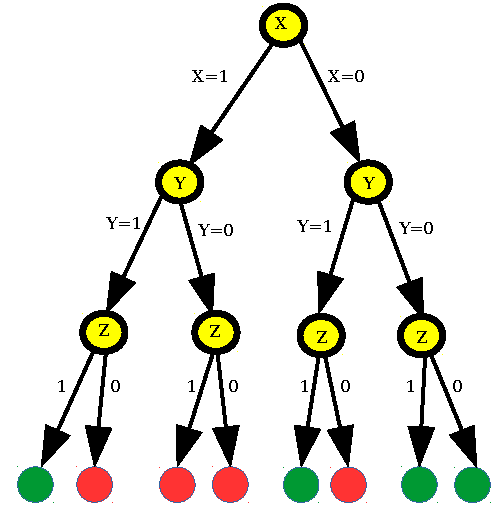
\includegraphics[width=0.8\textwidth , height=0.65\textheight]{xyz_tree.pdf}
 \caption{Representando as validades da função $\varphi_3 (x,y,z)$} 
%\label{}
\end{figure}

\end{frame}
%%%%%%%%%%%%%%%%%%%%%%%%%%%%%%%%%%%%%%%%%%%%%%%%%%%%%%%%%%%%%%%%%%%%


\subsection{Problema da Satisfatibilidade}

\begin{frame}[fragile]

\begin{block}{O que temos em comum entre $\varphi_1 (x)$, $\varphi_2 (x,y)$
$\varphi_3 (x,y,z)$?}
\pause
\begin{itemize}
  \item Claro, o mesmo domínio: $\{0,1\}$ 
  \item O número de linhas cresceu ....
  \pause
    \item Sim, o número de linhas cresceu e exponencialmente: \textbf{$2^{n}$} onde é o número
    de variáveis 
      \item Quanto a base $2$ veio tamanho do domínio: $\{0,1\}$
      \pause
      \item E quando este número de variáveis e domínio forem maiores?
\pause
      \item Isto mesmo, temos $\mid D\mid ^{n}$, \textcolor{red}{uma exponencial}!
\pause
  \item Logo, problemas que tenham uma ordem maior ou igual a {\Large \textbf{$2^{O(n)}$}}
  são \textcolor{red}{exponenciais}, consequentemente, \textcolor{red}{difíceis}!
  \end{itemize}

\end{block}

\end{frame}



\subsection{Classificação de Problemas}

\begin{frame}
\frametitle{Classe de Problemas e o interesse da IA}

\begin{figure}[ht!]
 \centering
 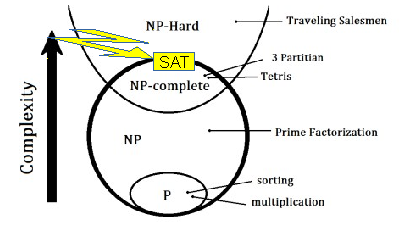
\includegraphics[width=0.8\textwidth , height=0.6\textheight]{classes_problemas.pdf}
 \caption{Problemas e suas complexidades} 
%\label{}
\end{figure}

\end{frame}






%%%%%%%%%%%%%%%%%%%%%%%%%%%%%%%%%%%%%%%%%%%%%%%%%%%%%%%
\section{Otimização Combinatória}

\frame{
    \frametitle{Introdução à Otimização}
    
    \begin{figure}[tbp]
%    \includegraphics[keepaspectratio=true,width=4in]{../res/opt_termos}
    \centering
    \end{figure}
}
%%%%%%%%%%%%%%%%%%%%%%%%%%%%%%%%%%%%%%%%%%%%%%%%%%%%%%%

\begin{frame}[fragile]
    \frametitle{Classes de Problemas}
    
    Problemas de otimização são geralmente divididos em dois tipos: \emph{otimização combinatorial} (\textit{discreta}) e
    \emph{otimização numérica} (\textit{contínua})
    \hspace{5em}
    \begin{description}
    \item[Combinatorial] Problemas definidos em um espaço de estados finito (ou infinito mas enumerável)
    \item[Numérica] Definidos em subespaços infinitos e não enumeráveis, como os números
    reais e complexos
    \end{description}
\end{frame}

%%%%%%%%%%%%%%%%%%%%%%%%%%%%%%%%%%%%%%%%%%%%%%%%%%%%%%%
\frame{
    \frametitle{Elementos de uma Otimização}
    
    \begin{figure}[tbp]
    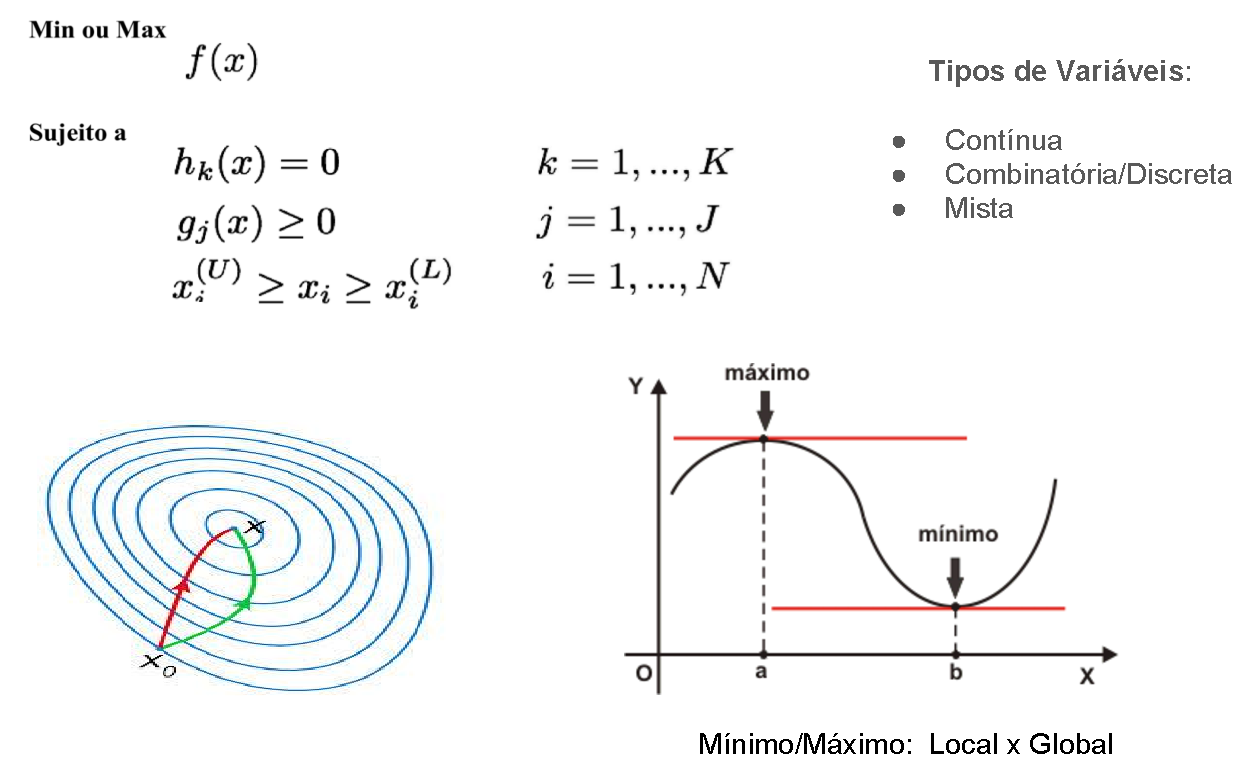
\includegraphics[keepaspectratio=true,width=4in]{elementos-da-otimizacao.pdf}
    \centering
  %%  \caption{Atribuição ou designação de trabalhos}
%    \label{fig:ex2}
    \end{figure}
}
%%%%%%%%%%%%%%%%%%%%%%%%%%%%%%%%%%%%%%%%%%%%%%%%%%%%%%%


%%%%%%%%%%%%%%%%%%%%%%%%%%%%%%%%%%%%%%%%%%%%%%%%%%%%%%%
\frame{
    \frametitle{Otimização Combinatorial - Exemplo}
    
    \begin{figure}[!tbp]
     \centering
%    \includegraphics[width=0.8\textwidth , height=0.6\textheight]{../res/des}

    \caption{Atribuição ou designação de trabalhos}
%    \label{fig:ex2}
    \end{figure}
}
%%%%%%%%%%%%%%%%%%%%%%%%%%%%%%%%%%%%%%%%%%%%%%%%%%%%%%%

\frame{
    \frametitle{Otimização Numérica - Exemplo}
    
    Minimizar a função $f(x) = (x-1)^{2} + 3$.
    
    \begin{figure}[!ht]
 %   \includegraphics[width=0.8\textwidth , height=0.6\textheight]{../res/min_num}
    \centering
    \end{figure}
 }
%%%%%%%%%%%%%%%%%%%%%%%%%%%%%%%%%%%%%%%%%%%%%%%%%%%%%%%
\begin{frame}[fragile]
 \frametitle{As técnicas:} 
  
\begin{block}{}
      \begin{description}
      \item[Combinatória:]
      \begin{itemize}
           \item Busca Local
          \item Métodos Gulosos: busca tipo subida a encosta (\textit{hill-climbing}), recozimento simulado (\textit{simulated annealing}), busca tabu, etc
        \item Programação Dinâmica
        \item \underline{\textbf{Programação por Restrições}}
        \item Redes de Fluxo
        \item .....        
        \end{itemize}      
      
      \item[Numérica:]
        \begin{itemize}
        \item Descida do Gradiente 
        \item Gauss-Newton
        \item Lavemberg-Marquardt
        \item .....
      \end{itemize}      
       
    \end{description}
  \end{block}
\end{frame}

%%%%%%%%%%%%%%%%%%%%%%%%%%%%%%%%%%%%%%%%%%%%%%%%%%%%%
\section{Um Exemplo de Problema Dificil: Cabo de Guerra}

\begin{frame}
\frametitle{Um Problema NP-Difícil: Cabo de Guerra}

\begin{figure}[ht!]
 \centering
 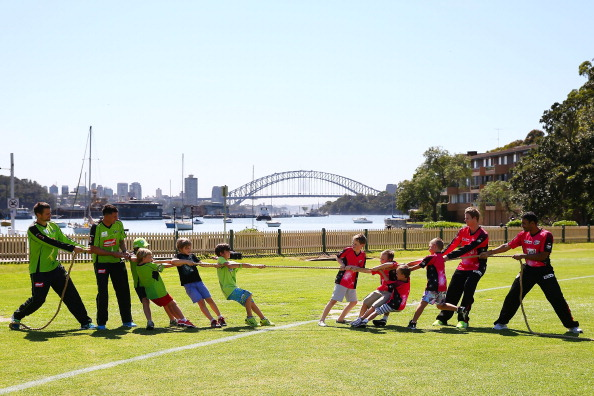
\includegraphics[width=0.8\textwidth , height=0.7\textheight]{cabo-de-guerra.jpg}
% \caption{} 
%\label{}
\end{figure}


\end{frame}

%%%%%%%%%%%%%%%%%%%%%%%%%%%%%%%%%%%%%%%%%%%%%%%%%%%%%%%%%%%%%%%%

\begin{frame}[fragile]
\frametitle{Critério de escolha do times: por peso}

\begin{figure}[ht!]
 \centering
 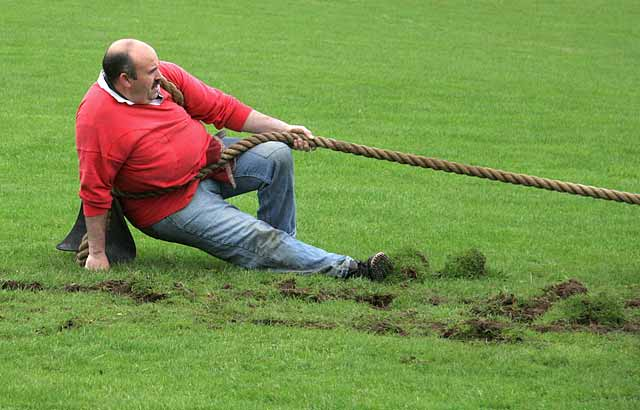
\includegraphics[width=0.7\textwidth , height=0.7\textheight]{separar_por_peso02.jpg}
\caption{\textit{O mais pesado tem mais força!}} 
%\label{}
\end{figure}

\end{frame}

%%%%%%%%%%%%%%%%%%%%%%%%%%%%%%%%%%%%%%%%%%%%%%%%%%%%%%%%%%%%%

\begin{frame}[fragile]%%%%%[allowframebreaks=0.9]
\frametitle{Especificando o problema}

\begin{block}{Que seja feita a divisão:}
 
\begin{center}
\begin{tabular}{|c|c|c|c|c|}
\hline
$Joao_1$ & $Pedro_2$ & $Manoel_3$ & .... & $Zeca_n$ \\ \hline
45 & 39 & 79 & .... & 42  \\ \hline
\end{tabular}
\end{center}

\begin{itemize}
\item Divisão  por peso
\item Respeitar  critérios como: $|N_A - N_B| \le 1$
\item Todos devem brincar

\item \textsf{Bem, esta simples {\bf \underline{restrição}} ({\bf $|N_A - N_B| \le 1$}), de nosso cotidiano tornou um simples problema em mais uma questão combinatória.
 Um arranjo da ordem de  $\frac{n!}{(n/2)!}$.
 Casualmente, nada trivial  para grandes valores! }
 \end{itemize}
 
\end{block}
\end{frame}
%%%%%%%%%%%%%%%%%%%%%%%%%%%%%%%%%%%%%%%%%%%%%%%%%


\subsection{Modelagem}

\begin{frame}[fragile]%%%%%[allowframebreaks=0.9]
\frametitle{Estratégia de Modelagem}
\begin{block}{Variável de Decisão $\Rightarrow $ análogo há um caminho na árvore de SAT}
  \begin{itemize}

\item Modelando:\\

\begin{tabular}{l|c|c|c|c|c}
\hline \hline
Nomes: & $Joao_1$ & $Pedro_2$ & $Manoel_3$ & .... & $Zeca_n$  \\ \hline
Peso ($p_i$): & 45 & 39 & 79 & .... & 42  \\ \hline
Dec. Binária ($x_i$): & $x_1$ & $x_2$ & $x_3$ & .... & $x_n$ \\ \hline
Dec. Binária ($x_i$): & 0/1 & 0/1 & 0/1 & .... & 0/1  \\ 
\hline \hline
\end{tabular}

\item $x_i = 0$: $n_i$ fica para o time $A$
\item $x_i = 1$: $n_i$ fica para o time $B$
  
  \end{itemize}
  
\end{block}
\end{frame}

%%%%%%%%%%%%%%%%%%%%%%%%%%%%%%%%%%%%%%%%%%%%%%%%%
\subsection{Modelagem}

\begin{frame}[fragile]%%%%%[allowframebreaks=0.9]
\frametitle{Modelagem das Restrições}
\begin{block} {}   %{Quanto as restrições:}
  \begin{itemize}
  \item $N_A \approx N/2$, $N_B \approx N/2$  e  $|N_A - N_B| \le 1$   

  \item O peso total é a soma de todos os pesos: $\sum_{i=1}^n  p_i$
  
  \item Quanto ao  peso do time $B$:
        $$P_B = \sum_{i=1}^n x_i p_i$$ pois define-se que quando $x_i=1$ é do time $B$

  \item Peso total do time $A$ ($P_A$) é dado por: $P_A = P_{total} - P_B$
  
  \item Ou $P_A = \sum_{i=1}^n p_i - \sum_{i=1}^n x_i p_i$

  \item Finalmente, aplicar uma minimização  na diferença: $|P_A - P_B|$
   
  \end{itemize}
\end{block}
\end{frame}

%%%%%%%%%%%%%%%%%%%%%%%%%%%%%%%%%%%%%%%%%%%%%%%%%
\subsection{Uma Estratégia de Implementação}

\begin{frame}[fragile]%%%[allowframebreaks=0.9]
\frametitle{Uma Estratégia de Implementação}

\begin{block}{Um vetor binário de $n$ posições representando a escolha de cada um no time:}

 \begin{center}

 \textbf{
 \begin{tabular}{|c|c|c|c|c|c|} 
 \hline
  $x_1: \textcolor{red}{0/1}$ & $x_2:\textcolor{red}{0/1}$ & $x_3:\textcolor{red}{0/1}$ & $x_4:\textcolor{red}{0/1}$ & .... & $x_n:\textcolor{red}{0/1}$  \\ \hline
  \end{tabular}
 } 
 \begin{itemize}

   \item  \textcolor{red}{Uma solução $=$ um caminho escolhido da raiz até uma das folhas da árvore de SAT}
  
\item Basta encontrar qual é a de melhor solução (eis a otimização)!

 \end{itemize}
 \end{center}
 
\end{block}

\end{frame}
  


\begin{frame}[fragile]%%%[allowframebreaks=0.9]
\frametitle{Uma árvore SAT com muitos caminhos ...}
  
\begin{figure}[ht!]
 \centering
 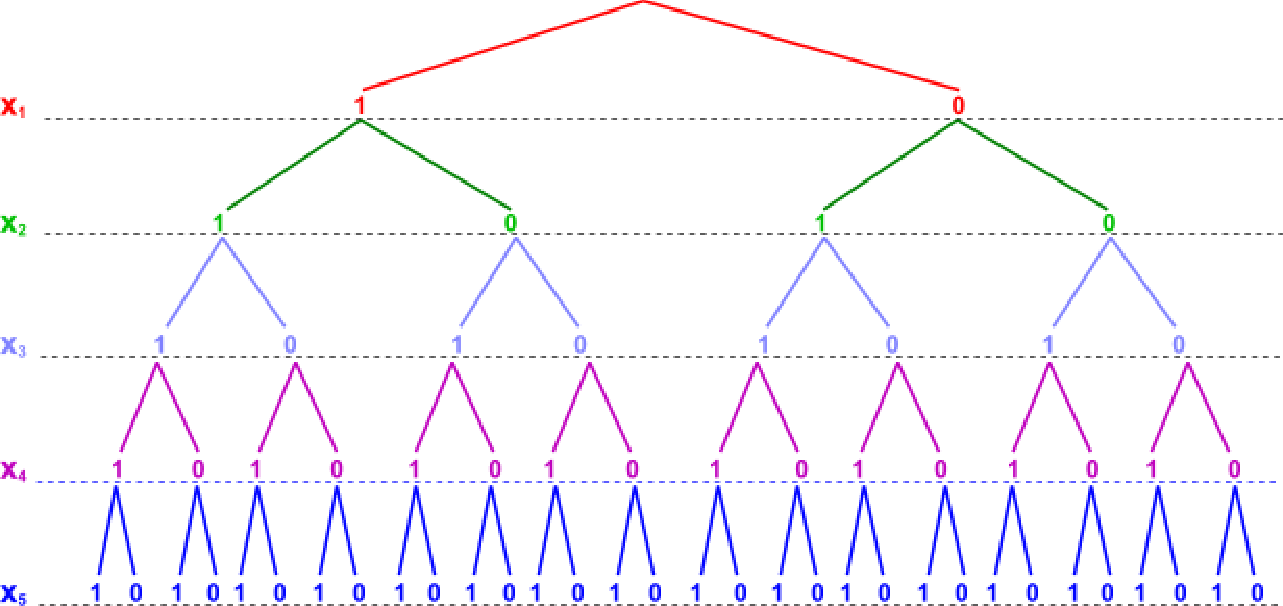
\includegraphics[width=0.8\textwidth , height=0.6\textheight]{binary_tree04.pdf}
\caption{Se $x_i=0$, então $n_i$ segue para o time $A$, caso  $x_i=1$, então  $n_i$ vai para o time $B$. Basta avaliar todos os caminhos e descobrir qual é o melhor!} 
%\label{}
\end{figure}

\end{frame}

%%%%%%%%%%%%%%%%%%%%%%%%%%%%%%%%%%%%%%%%%%%%%%%%%
\subsection{Implemetação em Minizinc}

\begin{frame}[allowframebreaks=0.9]
\frametitle{Implementação em Minizinc}

\lstinputlisting{minizinc/cabo_de_guerra.mzn}

\end{frame}

%%%%%%%%%%%%%%%%%%%%%%%%%%%%%%%%%%%%%%%%%%%%%%%%%

%%%%%%%%%%%%%%%%%%%%%%%%%%%%%%%%%%%%%%%%%%%%%%%%%

\subsection{Resultados e Análise}

\begin{frame}[fragile]
\frametitle{Resultados e Análise}

\begin{footnotesize}
\begin{verbatim}
Finished in 50msec
Compiling cabo_de_guerra.mzn
Running cabo_de_guerra.mzn
 Peso Total: 651	 PA : 312	 PB : 339
 Vetor de pesos: [77, 97, 120, 45, 57, 96, 100, 59]
 V_BIN_TIMES B/1 A/0: [1, 1, 1, 1, 0, 0, 0, 0]
----------
 Peso Total: 651	 PA : 332	 PB : 319
 Vetor de pesos: [77, 97, 120, 45, 57, 96, 100, 59]
 V_BIN_TIMES B/1 A/0: [0, 1, 1, 1, 1, 0, 0, 0]
----------
 Peso Total: 651	 PA : 324	 PB : 327
 Vetor de pesos: [77, 97, 120, 45, 57, 96, 100, 59]
 V_BIN_TIMES B/1 A/0: [1, 1, 0, 0, 1, 1, 0, 0]
 TIME A: [120, 45, 100, 59]
 TIME B: [77, 97, 57, 96]
----------
==========
\end{verbatim}

\end{footnotesize}

\end{frame}
%%%%%%%%%%%%%%%%%%%%%%%%%%%%%%%%%%%%%%%%%%%%%%%%%%%%%%%%
\begin{frame}[fragile]
\frametitle{Resultados e Análise}
\framesubtitle{Números aleatórios aos pesos: 1 a 150}
\begin{block}{
Usando um \textit{solver} médio do Minizinc (\textit{G12 lazyfd}) padrão:}
\begin{small}
\begin{center}
  \begin{tabular}{ l | c |c | r }
    \hline  \hline 
    $n$ & tempo & $P_A$ & $P_B$\\ \hline     \hline 
     5 & 40msec & 276 & 278 \\ \hline
    10 & 46msec & 518 & 519 \\ \hline
    25 & 98msec & 1198 & 1197 \\ \hline
    50 & 411msec & 2290 & 2291 \\ \hline
    75 & \textbf{\textcolor{red}{2s 485msec}} & 3133 & 3133 \\ \hline
    100 & 470msec & 4142 & 4142 \\ \hline 
    125 & \textbf{\textcolor{red}{7s 2msec}} & 4992 & 4992 \\ \hline 
    150 & 605msec & 5823 & 5823 \\ \hline 
    175 & 642msec &   6777 &  6778 \\ \hline 
    200 & $>$ 10min & -- & -- \\ \hline \hline
  \end{tabular}
\end{center}
\end{small}
Referência: cpu 4-core, 4 G ram, SO: Linux-Debian

\end{block}
\end{frame}

%%%%%%%%%%%%%%%%%%%%%%%%%%%%%%%%%%%%%%%%%%%%%%%%%%%%%%%



%%%%%%%%%%%%%%%%%%%%%%%%%%%%%%%%%%%%%%%%%%%%%%%%%%%%
\subsection{Resumindo ... }

\begin{frame}
\frametitle{Reflexões}
\begin{block}{}   %%%%Implemetação em Minizinc
\begin{flushleft}

\vspace{1cm}
\ding{224} \textsf{Enfim, este problema é uma variação de clássicos
NPs, mais especificamente o \textit{sub-set-sum}}

\vspace{1cm}
\ding{224} \textsf{Leia-se: Problema da Mochila}


\vspace{1cm}
\ding{224} \textsf{Implemente este problema usando Programação Dinâmica (PD)}

      \end{flushleft}

    \end{block}
  \end{frame}

%%%%%%%%%%%%%%%%%%%%%%%%%%%%%%%%%%%%%%%%%%%%%%%%%%%%%%%



\begin{frame}
\frametitle{Finalizando estes exponenciais}

\begin{figure}[h!b]
\begin{center}
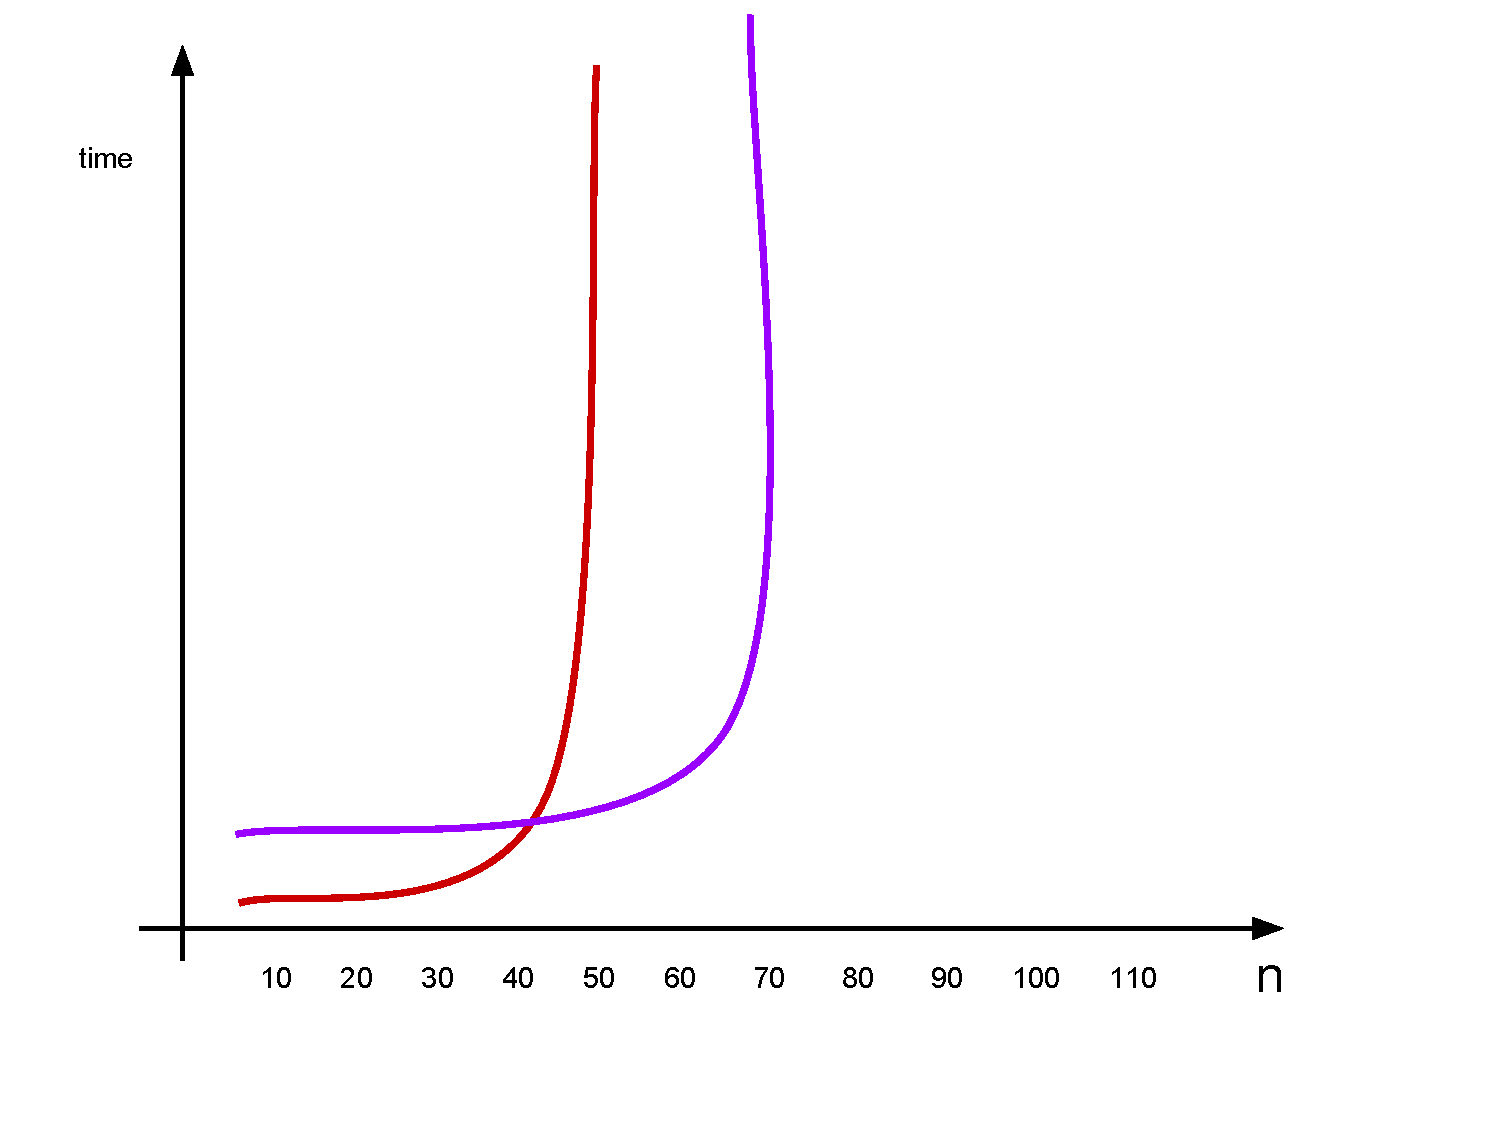
\includegraphics[width=0.7\textwidth , height=0.7\textheight]{Execution-Time-NP-01.pdf}
\caption{O limite dos NPs}
\label{fig_Execution-Time-NP-01}
\end{center}
\end{figure}

% 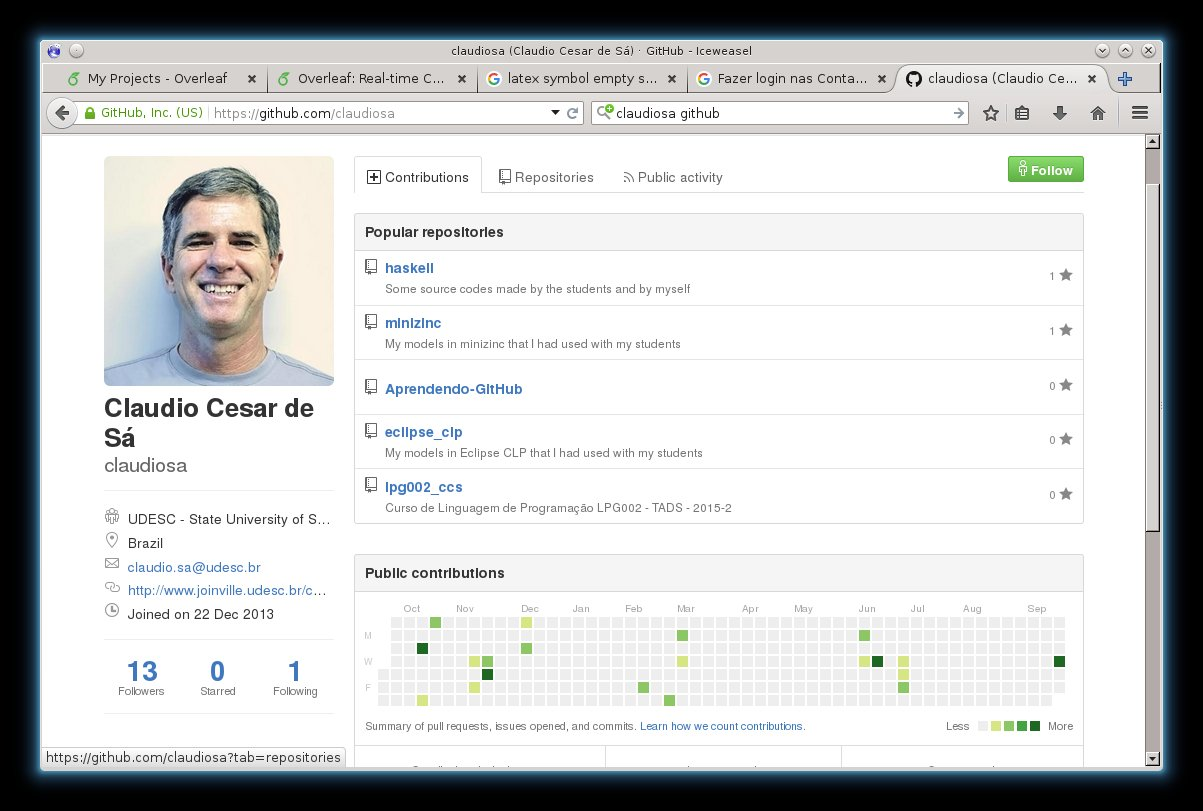
\includegraphics[width=0.7\textwidth , height=0.7\textheight]{meus-codigos-fontes.jpeg}

\end{frame}

%%%%%%%%%%%%%%%%%%%%%%%%%%%%%%%%%%%%%%%%%%%%%%%%%%%%%%%


\begin{frame}[fragile]
\frametitle{\textit{Empurrando} o \textit{muro} dos exponenciais}

\begin{figure}[!hb]
\begin{center}
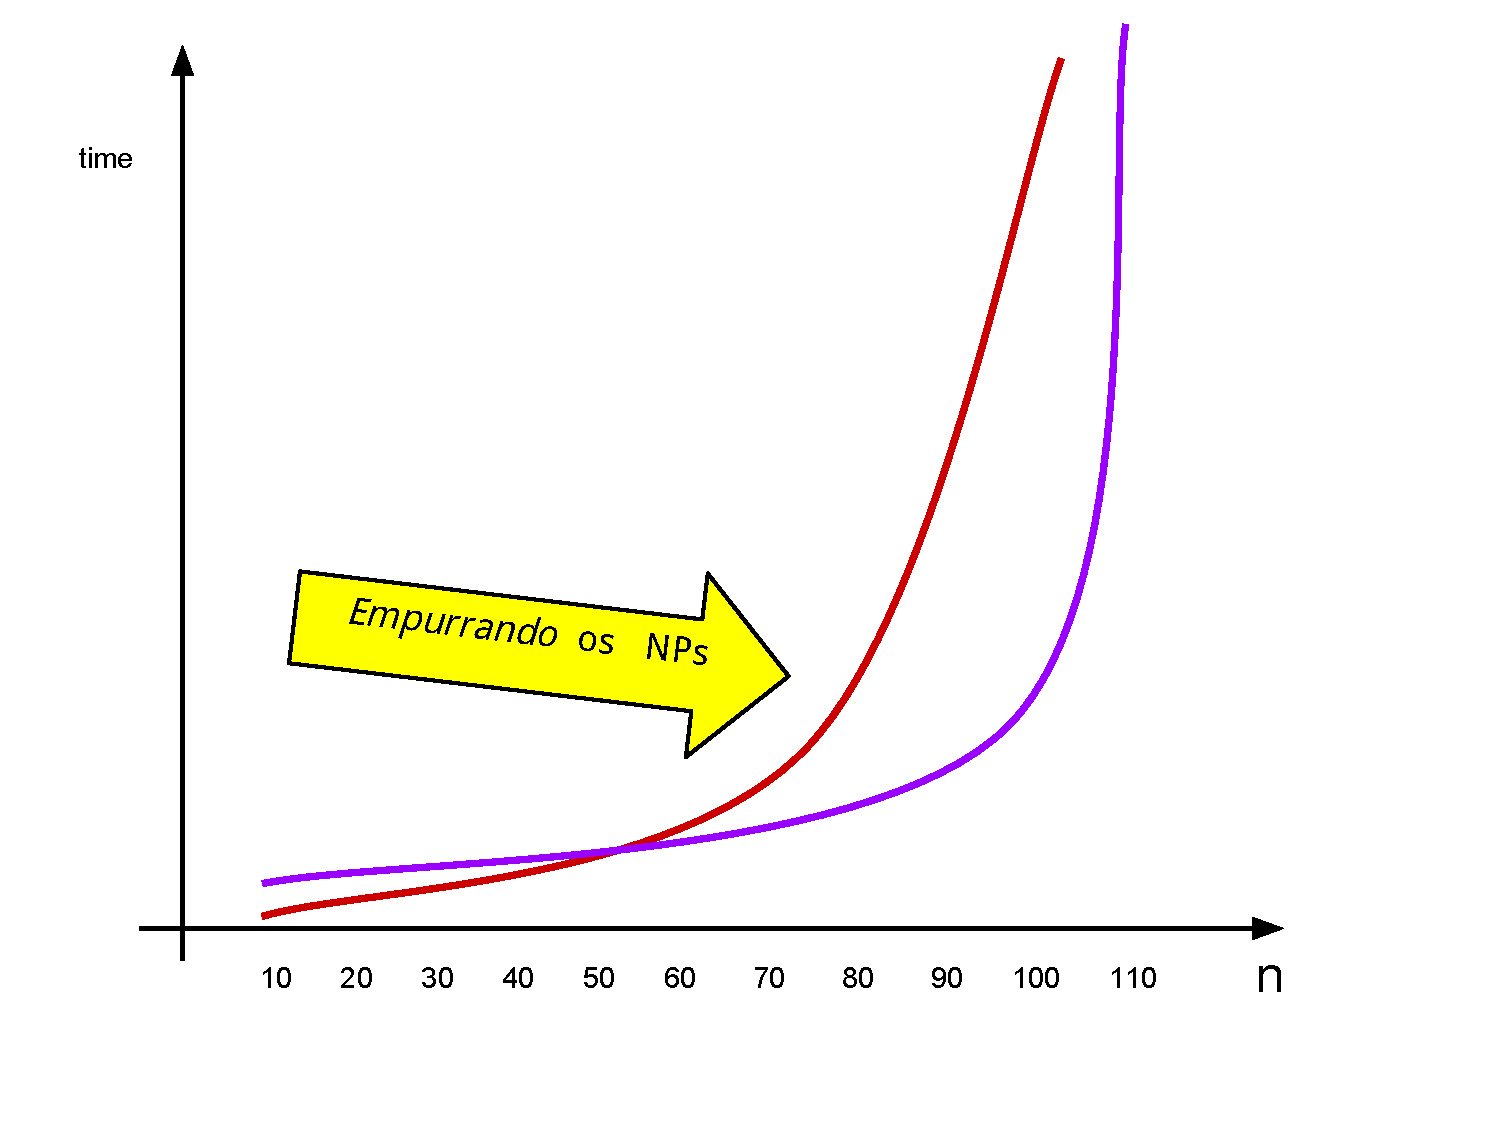
\includegraphics[width=0.7\textwidth , height=0.7\textheight]{Execution-Time-NP-03.pdf}
\caption{{\em Empurrando} o limite dos NPs}
\label{fig_Execution-Time-NP-03}
\end{center}
\end{figure}

% 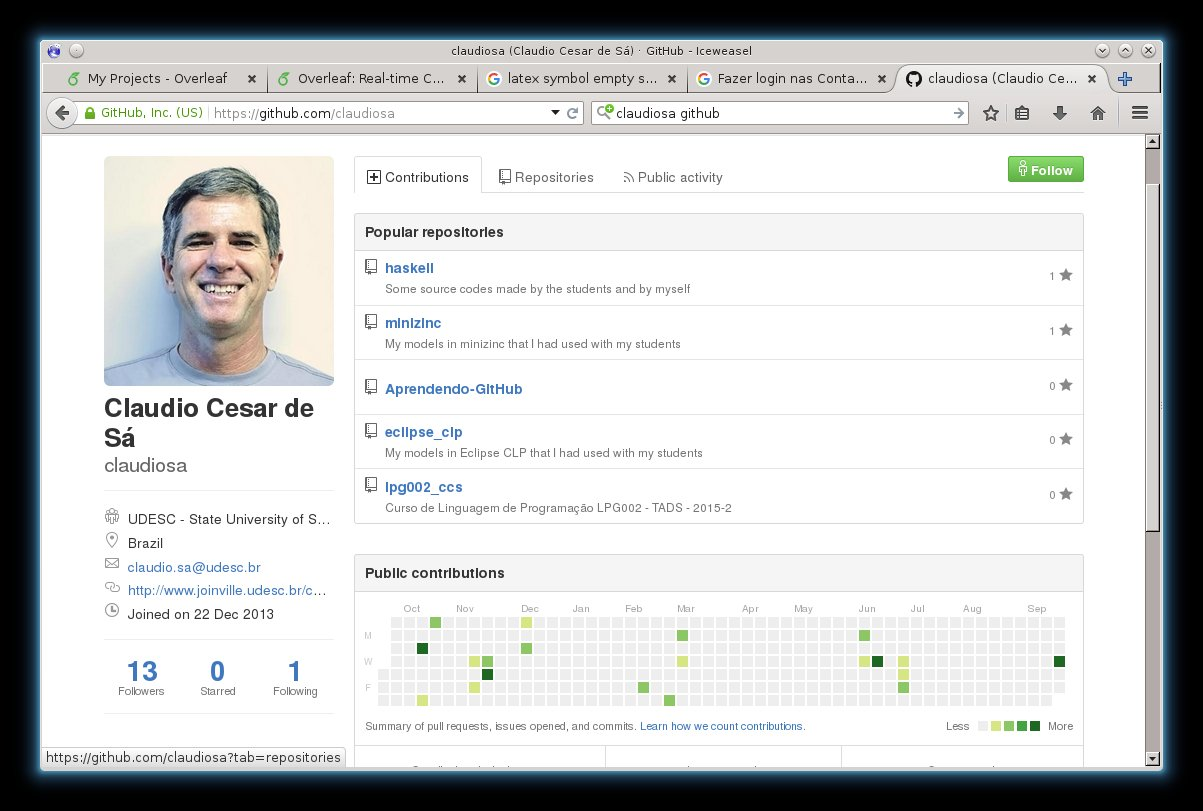
\includegraphics[width=0.7\textwidth , height=0.7\textheight]{meus-codigos-fontes.jpeg}

\end{frame}



\section{Conclusões}

\begin{frame}[fragile]%% [allowframebreaks=0.9]
\frametitle{Conclusões}
\begin{block}

  \begin{itemize}
  \item A área computação evolucionária tem apresentado resultados expressivos,   são resultados \textit{quase-ótimos}, mas magnetudes acima das demais técnicas;
  \pause
    
  \item O hardware com IA embarcada sempre foi um paradigma da construção   de uma \textit{inteligência}
    \pause
    
  \item Os \textit{rápidos}, \textit{baratos} e \textit{velozes}, agora formam   um sociedade de agentes inteligentes
    \pause
    
  \item Os problemas solucionados com a \textit{combinatória} tem sido colocados em prática   há muitos anos, e ao que parece, devem continuar, ....
    \pause
  
  \item Mas, a nível de Brasil, estamos tímidos!
  
  \end{itemize}
  \end{block}

\end{frame}

%%%%%%%%%%%%%%%%%%%%%%%%%%%%%%%%%%%%%%%%%%%%%%%%%%%%%%%


\section{Agradecimentos e Referências}

\begin{frame} [allowframebreaks=0.9]
\frametitle{Perguntas e Referências}
  
  \begin{center}
%   
\includegraphics[scale=0.6,keepaspectratio]{simpsons.jpg} 
   
\includegraphics[scale=0.35,keepaspectratio]{test_intelligence01.jpg} 
  \end{center} 

\vspace{-1cm}

\begin{block}{}
  % Keep the summary *very short*.
  \begin{itemize}
  \item \url{http://www.joinville.udesc.br/coca/}
  
  \item \url{https://github.com/claudiosa}

  \item Email: \url{claudio.sa@udesc.br}


  \item \textit{Thank you so much}!

  \end{itemize}
  \end{block}

\end{frame}


%%%%%%%%%%%%%%%%%%%%%%%%%%%%%%%%%%%%%%%%%%%%%%%%%%%%%%%



\end{document}
